\section{10.2 - Optimal Control of Pitch/Travel without Feedback }

\subsection{The continuous model}
\textit{Answer 10.2.1.1}
The model is shown below. It does not only model the helicopter, but also the regulator in closed loop.

\[\begin{bmatrix}
    \dot\lambda \\ \dot{r} \\ \dot{p} \\ \ddot{p}
\end{bmatrix} =
\begin{bmatrix}
    0 & 1 & 0 & 0 \\
    0 & 0 & -K_2 & 0 \\
    0 & 0 & 0 & 1 \\
    0 & 0 & -K_1K_{pd} & -K_1K_{pp} 
\end{bmatrix}
\begin{bmatrix}
    \lambda \\ r \\ p \\ \dot{p}
\end{bmatrix}+
\begin{bmatrix}
    0 \\ 0 \\ 0 \\ K_1K_{pp}
\end{bmatrix}p_c\]

\subsection{The discretized model}
\textit{Answer 10.2.1.2. Remember to document the calculations.}

\[
A=
\begin{bmatrix}
    1 & 0.25 & 0 & 0 \\
    0 & 1 & -0.1415 & 0 \\
    0 & 0 & 1 & 0.25 \\
    0 & 0 & -0.81 & 0.1 
\end{bmatrix},
B=
\begin{bmatrix}
    0 \\ 0 \\ 0 \\ 0.81
\end{bmatrix}
\]

\begin{figure}[h]
    \centering
    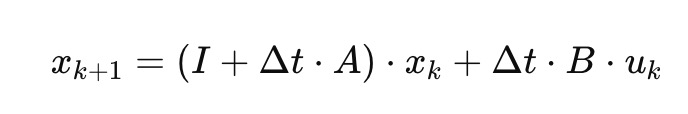
\includegraphics[width=0.6\linewidth]{Rapport/figures/Screenshot 2024-02-20 at 14.17.21.jpg}
    \caption{euler discreete.}
    \label{fig:enter-label}
\end{figure}

\subsection{The open loop optimization problem}
\textit{How is it formulated?}

\subsection{The weights of the optimization problem}
\textit{Plot both the state and input trajectories for the various weights, q. Comment the results with respect to the different weights chosen.}
\textit{If you have answered the "For the daring" questions from 10.2.1.3, include the answer here.}

\subsection{Experimental results}
\textit{Printouts of data from relevant experiments (plots).
Discussion and analysis of the results.
Answer 10.2.2.7 here.}

\subsection{MATLAB and Simulink}
\textit{Code and diagrams go here (only lines that you've written yourself). Give some explanation of the code if necessary.}
	
	
	
	
	
	
	
	
	
	
	
	
	 
	
